\chapter{Planteamiento del Problema}
\section{Descripción de la Realidad Problemática}

En la actualidad, cada vez es más necesario el uso de la conectividad a internet como método de interacción entre los usuarios, empresas e instituciones educativas, convirtiéndose en un instrumento imprescindible para las actividades relacionadas a ella. En la mayoría de las empresas no se cuenta con una cobertura de la red Wi-Fi total que garantice el acceso a internet y es allí donde surgen muchos inconvenientes tanto para el envío de trabajos, realización de consultas, entre otras actividades en las que la red sería de gran ayuda.

Lograr encontrar la ubicación idónea de Aps Indoor para lograr la cobertura total de un lugar es un proceso iterativo que consume mucho tiempo, que requiere múltiples rondas de refinamientos. Un especialista de TI esboza un diseño, evalúa, ajusta y repite los ciclos hasta estar satisfecho con un diseño dentro de un presupuesto de tiempo dado. Desafortunadamente, diseñar un plano de cobertura de red efectivo solo es posible mediante especialistas de TI o Redes, donde gran parte de empresas hacen su propio diseño personalizado menos efectivo debido al costo. La generación automática de planos de cobertura de red con las ubicaciones de Aps Indoor tendrá un tremendo impacto en las industrias de bienes raíces/construcción, redes y TI de billones de dólares.

En los últimos años, ha habido un aumento en la demanda de redes inalámbricas entre los usuarios, gracias a los beneficios que ofrecen en términos de movilidad y costos de implementación más bajos. Dentro de las redes inalámbricas, se encuentran las WLAN (Redes de Área Local Inalámbricas), las cuales son comúnmente utilizadas en entornos cotidianos como hogares, oficinas y instituciones educativas, entre otros lugares. Estas redes suelen estar compuestas principalmente por dispositivos concentradores conocidos como Puntos de Acceso (AP), los cuales permiten a los usuarios conectarse de forma inalámbrica a la red, cumpliendo una función similar a la de un Switch en una red cableada. Sin embargo, a pesar de la capacidad de los AP para establecer conexiones inalámbricas, la distancia efectiva entre el usuario y el AP es limitada (generalmente inferior a 100 metros), debido a la potencia de la señal de transmisión y a posibles obstáculos en el entorno que puedan afectar la señal. Debido a la creciente necesidad de conectividad inalámbrica por parte de los usuarios, la cantidad de Puntos de Acceso en uso está en constante aumento.

Según una investigación realizada por ABI Research, compañía que asesora a fabricantes del mundo de los semiconductores sin cable, en 2026 se llegará al despliegue total de Wi-Fi 6, el cual se acelera rápidamente mucho más allá de los dispositivos Wi-Fi insignia, cada vez más dispositivos admiten la banda de 6 GHz está integrado en un número cada vez mayor de dispositivos de consumo convencionales. \cite{ot_zig2020abi} Ello es algo que se debe tener, en cuenta debido al rápido avance de la tecnología y a las consecuencias que estas tendrán.

En un artículo del diario El País, se destaca un problema creciente relacionado con la conectividad Wi-Fi en los hogares. A medida que más dispositivos se conectan a las redes inalámbricas, la infraestructura existente se ve sometida a una presión cada vez mayor. Además, muchos hogares y empresas aún utilizan enrutadores y puntos de acceso antiguos que no pueden manejar la cantidad de dispositivos conectados, sumando la falta de actualización de la infraestructura contribuye al problema. \cite{ot_elpais2023wifi}

En el primer trimestre de 2022, el 95.0\% de los hogares del país contaban con al menos un servicio de Tecnología de Información y Comunicación (TIC), según el Instituto Nacional de Estadística e Informática (INEI). Este dato representa un aumento de 0,2 puntos porcentuales en comparación con el mismo trimestre de 2021 y 2019, respectivamente.  \cite{ot_inei2022estati}

En el ámbito de las redes inalámbricas, especialmente en entornos corporativos y de alta demanda, como los clientes de Cisco, las quejas sobre la conectividad y el rendimiento de las WLAN (Wireless Local Area Network) son una constante preocupación. A medida que aumenta la dependencia de estas redes para la comunicación, colaboración y operaciones empresariales, también lo hacen los desafíos técnicos y las expectativas de los usuarios. Uno de los problemas recurrentes es la cobertura inalámbrica insuficiente, que se manifiesta en áreas muertas donde la señal es débil o inexistente. Esto puede deberse a la ubicación subóptima de los puntos de acceso (AP) o a interferencias externas que obstaculizan la propagación de la señal. Los clientes de Cisco a menudo expresan su frustración por tener que moverse dentro de un espacio para obtener una señal sólida, lo que afecta negativamente la productividad y la experiencia del usuario.  \cite{ot_cisco2022ap}

\begin{figure}[h]
	\begin{center}
		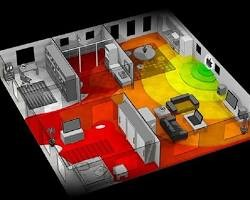
\includegraphics[width=0.55\textwidth]{1/figures/CISCO_QUEJAS.jpg}
		\caption[Quejas de Clientes en el foro de Cisco]{Quejas de Clientes en el foro de Cisco\\
		Fuente: \cite{ot_cisco2022ap}. \textit{Cobertura de red ineficiente}}
		\label{1:fig1}
	\end{center}
\end{figure}

Además de este problema, en muchos casos los usuarios optan por adquirir un nuevo punto de acceso para mejorar el medio ambiente, pero esto puede tener consecuencias negativas. La compatibilidad entre los dispositivos instalados no siempre está garantizada y también puede haber incompatibilidades a nivel de switch y VPN. Identificar y resolver estos problemas de una manera que tenga o tenga menos impacto en las operaciones requiere un sólido conocimiento técnico en el campo de las tecnologías de la información (TI), ya sea dentro del negocio o mediante el uso de servicios tecnológicos especializados. El procesamiento lento genera, entre otras desventajas, la necesidad de retrabajo, demoras en la emisión de informes y documentos y costos adicionales relacionados con las horas extras.  \cite{ot_napit2017ap}

A lo anterior, podemos sumar que los errores de configuración en switches, enrutadores y puntos de acceso también pueden tener un impacto negativo en la red inalámbrica, provocando, por ejemplo, ralentizaciones y caídas de conexiones. Por lo tanto, reconfigurar estos dispositivos puede ayudar a abordar los desafíos de la red. Una solución eficaz a esta situación es realizar un análisis detallado del entorno y las estructuras existentes. Con esta evaluación, resulta más fácil determinar la ubicación adecuada para conectar los elementos, evaluar los requisitos de los nuevos componentes y garantizar que sigan funcionando de manera óptima.  \cite{ot_napit2017ap}

\begin{figure}[h]
	\begin{center}
		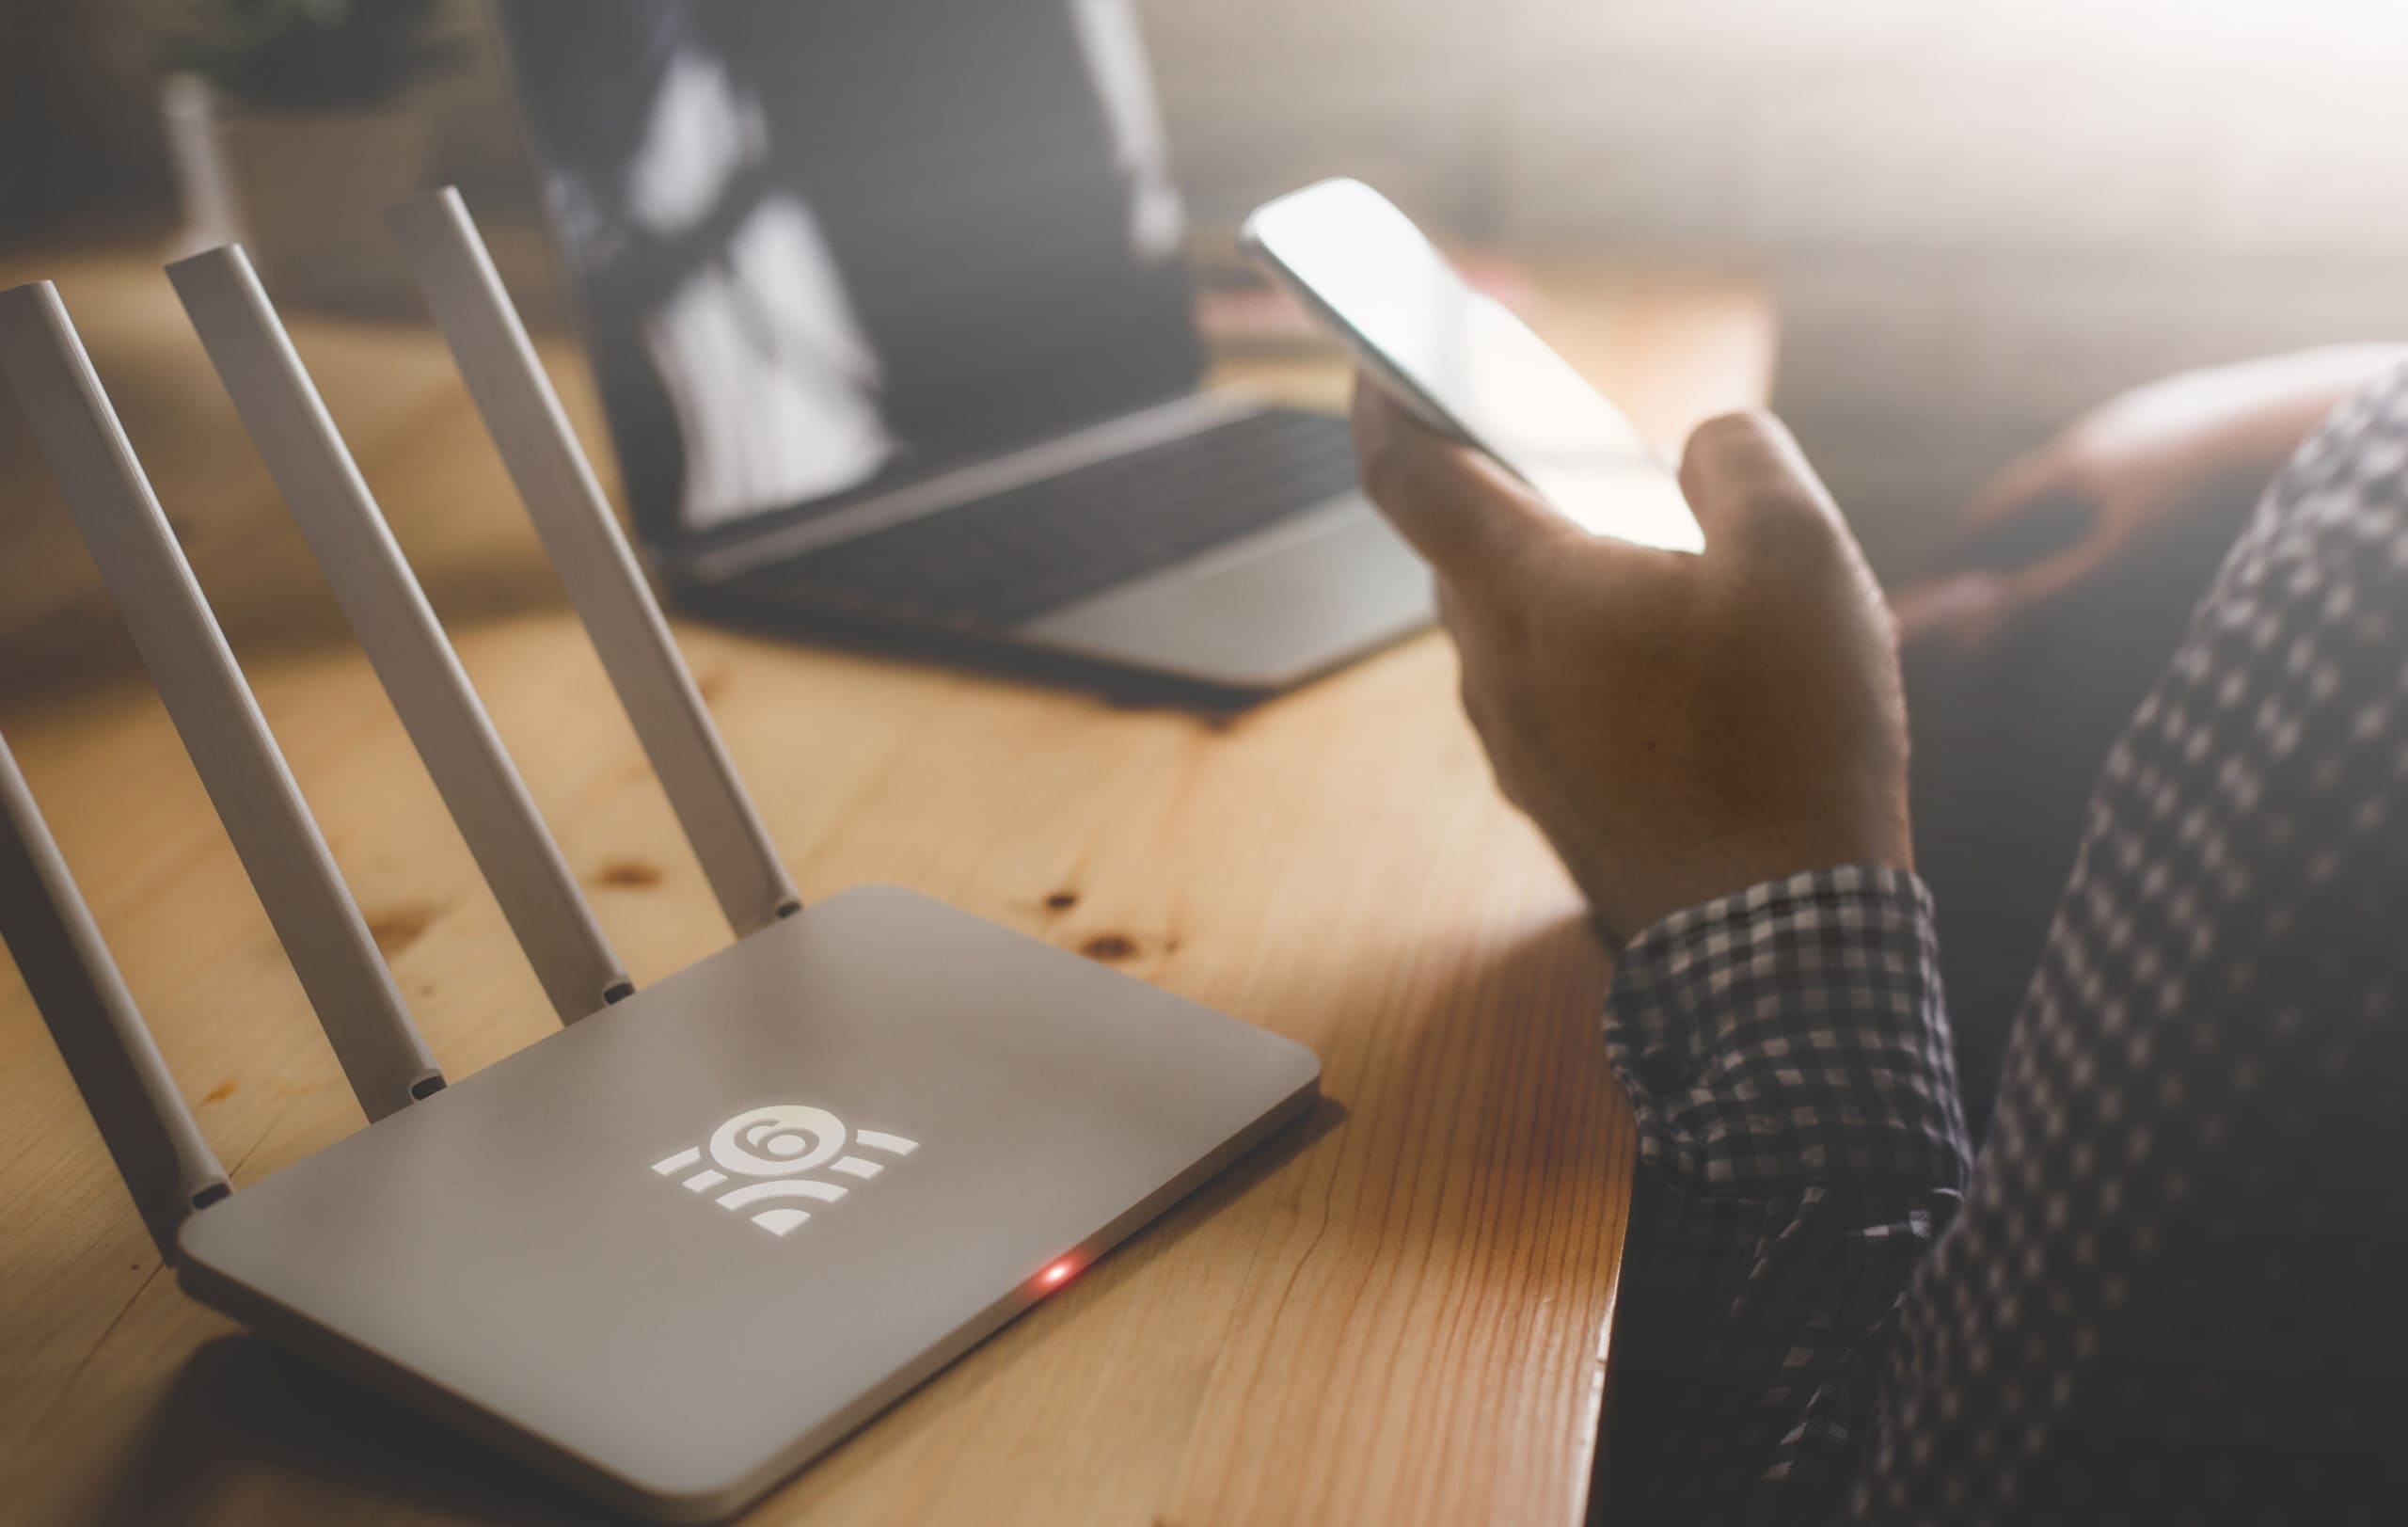
\includegraphics[width=0.55\textwidth]{1/figures/access-point-1.jpeg}
		\caption[Problemas de uso de Access Points]{Problemas de uso de Access Points\\
		Fuente: \cite{ot_napit2017ap}. \textit{Problema con el funcionamiento ideal del Access Point}}
		\label{1:fig2}
	\end{center}
\end{figure}

\section{Formulación del Problema}
Se creó un "árbol de problemas" para formular los problemas de la investigación actual. (Anexo 1: \ref{anexo1})

\subsection{Problema General}
PG: \newcommand{\ProblemaGeneral}{
¿Es posible predecir las ubicaciones de Puntos de Acceso (APs) Indoor en Diferentes Planos  mediante Inteligencia Artificial Generativa?
}
\ProblemaGeneral
\subsection{Problemas Específicos}
\newcommand{\Pbone}{
¿Cómo se puede modelar de manera efectiva la distribución espacial de usuarios y obstáculos en un entorno interior para predecir la cobertura inalámbrica?
}
\newcommand{\Pbtwo}{
¿Qué enfoques de inteligencia artificial generativa son más adecuados para generar ubicaciones óptimas de APs en entornos interiores?
}
\newcommand{\Pbthree}{
¿Cómo puedo encontrar una base de datos eficiente y robusta que almacene información detallada y precisa sobre la infraestructura de edificios y características de entornos indoor?
}
\newcommand{\Pbfour}{
¿Cuáles son las métricas y metodologías de evaluación más adecuadas para medir la eficiencia y efectividad de las predicciones de ubicaciones óptimas de puntos de acceso (APs) generadas por modelos de inteligencia artificial generativa en entornos indoor?
}

\begin{itemize}
	\item PE1: {\Pbone}
	\item PE2: {\Pbtwo}
	\item PE3: {\Pbthree}
	\item PE4: {\Pbfour}
\end{itemize}

\section{Objetivos de la Investigación}
Se creó un "árbol de objetivos" para establecer los objetivos de esta investigación. (Anexo 2: \ref{anexo2})
\subsection{Objetivo General}
OG: \newcommand{\ObjetivoGeneral}{
Desarrollar técnicas de inteligencia artificial generativa para predecir las ubicaciones óptimas de puntos de acceso (APs) en diferentes planos de un entorno interior, con el fin de optimizar la cobertura de redes inalámbricas y mejorar la conectividad y calidad del servicio para los usuarios finales.
}
\ObjetivoGeneral
\subsection{Objetivos Específicos}
\newcommand{\Objone}{
Desarrollar un algoritmo que pueda simular con precisión la cobertura de redes inalámbricas en interiores
}
\newcommand{\Objtwo}{
Implementar un modelo generativo capaz de proponer automáticamente ubicaciones eficientes para los Aps
}
\newcommand{\Objthree}{
Encontrar una base de datos eficiente y robusta que almacene información detallada sobre la infraestructura de los edificios y características de los entornos indoor.
}
\newcommand{\Objfour}{
Desarrollar un conjunto de métricas y un marco de evaluación para medir la eficiencia y efectividad de las predicciones generadas por los modelos de inteligencia artificial generativa en la optimización de la cobertura de redes inalámbricas indoor.
}

\begin{itemize}
	\item OE1: {\Objone}
	\item OE2: {\Objtwo}
	\item OE3: {\Objthree}
	\item OE4: {\Objfour}
\end{itemize}

\section{Hipótesis}

\subsection{Hipótesis General}
HG: \newcommand{\HipotesisGeneral}{
	La aplicación de técnicas de inteligencia artificial generativa para la predicción de la ubicación de puntos de acceso (Aps) en planes distribuidos en zonas interiores supone una mejora significativa en la cobertura y calidad del servicio de los recursos sin datos.
}
\HipotesisGeneral
\subsection{Hipótesis Específicas}
\newcommand{\Hone}{
	Los algoritmos de inteligencia artificial generativa, como las GAN, se pueden utilizar para predecir con precisión la ubicación óptima de los puntos de acceso (AP) en un entorno interior. 
}
\newcommand{\Htwo}{
	La combinación de datos de sensores de señales inalámbricos con datos como planos arquitectónicos mejoran la precisión y predicción de la ubicación de AP mediante inteligencia artificial generativa.
}
\newcommand{\Hthree}{
	Una base de datos bien gestionada y enriquecida con datos contextuales permitirá validar las predicciones de los modelos de IA de manera más fiable, comparando las ubicaciones sugeridas con las condiciones reales y mejorando la precisión de futuras predicciones.
}
\newcommand{\Hfour}{
	La implementación de un marco de evaluación estandarizado permitirá comparar de manera objetiva diferentes enfoques y modelos de IA, facilitando la selección de los más efectivos para optimizar la cobertura de redes inalámbricas en distintos entornos indoor.
}

\begin{itemize}
	\item HE1: \Hone
	\item HE2: \Htwo
	\item HE3: \Hthree
	\item HE4: \Hfour
\end{itemize}

La Matriz de Consistencia del Anexo 3 (\ref{anexo3}) alinea los problemas, objetivos e hipótesis mencionados anteriormente. Además, después de revisar los objetivos planteados en los antecedentes, cuyo detalle y referencia se encuentran en el Anexo 5 (\ref{anexo5}), se crearon los objetivos específicos a partir de una lluvia de ideas.

\section{Justificación de la Investigación}

\subsection{Teórica}
Los estudios teóricos sobre la optimización de la cobertura de redes inalámbricas mediante inteligencia artificial generativa se justifican por la necesidad de desarrollar soluciones eficaces, según \cite{pr_nauata2021housegan}, para entornos interiores donde se requieren muchas conexiones. La aplicación de algoritmos generativos brinda la oportunidad de mejorar la precisión del posicionamiento de los puntos de acceso (AP), reducir los costos operativos y garantizar una experiencia de usuario satisfactoria al minimizar las áreas de sombra y mantener una conexión estable. Estos avances son críticos en un contexto donde la conectividad inalámbrica es esencial para la productividad y disponibilidad de servicios digitales en planos complejos. 

El objetivo del estudio no es sólo mejorar la cobertura y calidad del servicio de la red inalámbrica, sino también optimizar los recursos y el gasto relacionado en infraestructura nacional. Se espera que mapear las capacidades de la IA generativa mejore significativamente el rendimiento de la red inalámbrica, la satisfacción del usuario y la adaptabilidad en espacios donde la conectividad confiable es esencial para la vida cotidiana y los negocios, como lo menciona el antecedente de \cite{pr_alathari2023optaps}.

\subsection{Práctica}
La investigación práctica sobre la optimización de la cobertura inalámbrica mediante inteligencia artificial generativa es crucial para garantizar la viabilidad y eficacia de las soluciones propuestas en entornos reales. Se pueden utilizar pruebas y experimentos prácticos para evaluar el uso de algoritmos generativos para predecir la ubicación de puntos de acceso (AP) en diferentes planos. Estos estudios proporcionan datos empíricos sobre mejoras en la cobertura, la eficiencia de los recursos y la calidad del servicio, proporcionando una base sólida para la adopción y expansión de estas tecnologías en el campo inalámbrico.

También participa en el desarrollo de herramientas y métodos aplicables a la industria de las telecomunicaciones y la gestión de redes. Trabajando con casos reales y diferentes entornos, es posible identificar desafíos específicos, optimizar algoritmos y proponer mejores prácticas para diseñar y optimizar redes inalámbricas en entornos interiores. Estos resultados son útiles para los investigadores de telecomunicaciones, pero también tienen implicaciones directas para mejorar la conectividad y la experiencia del usuario en diversos sectores, como empresas, instituciones educativas y espacios públicos.

\subsection{Metodológica}
La aplicación del modelo de inteligencia artificial generativa propuesto en este estudio ayuda a optimizar la cobertura de redes inalámbricas en ambientes interiores. Este modelo utiliza técnicas avanzadas de inteligencia artificial generativa, como las redes generativas adversarias (GAN) para predecir con precisión los puntos de acceso (AP) óptimos en diferentes niveles. La combinación de sensores de señal inalámbricos y una estructura de datos estructurados mejora significativamente la calidad del servicio y reduce los costos operativos asociados con la instalación y mantenimiento de la infraestructura de red.

Es por ello que este estudio puede proporcionar soluciones de datos efectivas, mejorar la conectividad inalámbrica en entornos interiores complejos. Al confirmar la aplicación de algoritmos generativos en el mundo real, este estudio proporciona una base sólida para la adopción y expansión de estas técnicas en la industria de las telecomunicaciones. Esto beneficia tanto a los usuarios finales, que garantizan una experiencia de usuario superior, como a las empresas, reduciendo costes y optimizando la eficiencia de las infraestructuras de redes inalámbricas.

\section{Delimitación del Estudio}

\subsection{Espacial}
Esta investigación se centra en optimizar la cobertura de la red inalámbrica en entornos interiores específicos como entornos comerciales, institucionales o residenciales. La investigación se lleva a cabo en áreas edificadas o construidas donde la conectividad inalámbrica es esencial para el funcionamiento eficiente de dispositivos y servicios. 

\subsection{Temporal}
El estudio cubre los últimos cinco años desde el año en curso 2024. Esto permite el uso de información actualizada y relevante para entrenar modelos creativos de IA y evaluar su efectividad para predecir la ubicación de puntos de acceso en diferentes niveles en un ambiente interior.

\subsection{Conceptual}
Esta investigación se orientará en técnicas de inteligencia artificial generativa, como las redes generativas adversarias (GAN) para optimizar la cobertura de la red inalámbrica. Se utilizan datos de sensores de señales inalámbricas, datos de construcción (por ejemplo, planos arquitectónicos) y técnicas de procesamiento de datos para mejorar la precisión de la predicción de la ubicación de la estación base y mejorar así la calidad del servicio de las redes inalámbricas en entornos interiores.